\documentclass[11pt,a4paper]{report}
% ============================================================
% PACKAGES
% ============================================================
\usepackage[utf8]{inputenc}
\usepackage[T1]{fontenc}
\usepackage{amsmath,amssymb}
\usepackage{graphicx}
\usepackage[american]{circuitikz}
\usepackage{tikz}
\usetikzlibrary{positioning,shapes,arrows.meta,calc}
\usepackage{pgfplots}
\usepgfplotslibrary{groupplots}
\usepackage{geometry}
\geometry{a4paper,margin=2.5cm}
\usepackage{fancyhdr}
\usepackage{titlesec}
\usepackage{enumitem}
\usepackage{booktabs}
\usepackage{longtable}
\usepackage{array}
\usepackage{xcolor}
\usepackage[colorlinks=true,linkcolor=blue,citecolor=blue,urlcolor=blue]{hyperref}
\usepackage{tcolorbox}
\tcbuselibrary{skins,breakable}
\usepackage{float}
\usepackage{caption}
\usepackage{multirow}
\usepackage{pifont}
\usepackage{siunitx}
\usepackage{hyperref}
\usepackage{subcaption}
\usepackage{import}
\usepackage{subcaption}
% ============================================================
% PAGE STYLE
% ============================================================
\pgfplotsset{compat=1.17}
\pagestyle{fancy}
\fancyhf{}
\fancyhead[L]{\small Analog Electronics Lab (PCEEL308)}
%\fancyhead[R]{\small \leftmark}
\fancyfoot[L]{Department of Electrical \& Electronics Engineering | GEC Barton Hill}
\fancyfoot[R]{\thepage}
\renewcommand{\headrulewidth}{0.4pt}

\titleformat{\chapter}[display]
  {\normalfont\bfseries\Large}
  {\chaptertitlename\ \thechapter}{10pt}{\Huge}
\titleformat{\section}{\normalfont\bfseries\large}{\thesection}{1em}{}

% ============================================================
% CUSTOM BOXES
% ============================================================
\newtcolorbox{safetybox}[1][]{
  colback=red!5!white,
  colframe=red!60!black,
  fonttitle=\bfseries,
  title=\ding{43}\ Safety Note,
  breakable,#1
}
\newtcolorbox{aimbox}[1][]{
  colback=blue!4!white,
  colframe=blue!40!black,
  fonttitle=\bfseries,
  title=Aim,
  breakable,#1
}
\newtcolorbox{prelabbox}[1][]{
  colback=yellow!8!white,
  colframe=yellow!50!black,
  fonttitle=\bfseries,
  title=Pre-Lab Assignment,
  breakable,#1
}
\newtcolorbox{precautionbox}[1][]{
  colback=orange!6!white,
  colframe=orange!70!black,
  fonttitle=\bfseries,
  title=Precautions,
  breakable,#1
}
\newtcolorbox{notebox}[1][]{
	colback=green!6!white,
	colframe=green!70!black,
	fonttitle=\bfseries,
	title=Note,
	breakable,#1
}
\newtcolorbox{explorebox}[1][]{
	colback=green!6!white,
	colframe=green!70!black,
	fonttitle=\bfseries,
	title=Explore further,
	breakable,#1
}
% Placeholder for figures -- replace \fig{caption}{label}{width} with actual
% \includegraphics or circuitikz code as the manual is developed.
\newcommand{\figplaceholder}[3][0.6\textwidth]{%
  \begin{figure}[H]
    \centering
    \fbox{\parbox[c][4cm][c]{#1}{\centering \textit{Figure Placeholder:}\\ #2}}
    \caption{#2}
    \label{#3}
  \end{figure}
}

% Placeholder for observation tables
\newcommand{\tableplaceholder}[2]{%
  \begin{table}[H]
    \centering
    \caption{#1}
    \label{#2}
    \renewcommand{\arraystretch}{1.6}
    \begin{tabular}{cccc}
      \toprule
      \textbf{Sl. No.} & & & \\
      \midrule
       & & & \\ 
       & & & \\ 
       & & & \\ 
      \bottomrule
    \end{tabular}
  \end{table}
}

\newcommand{\circuitplaceholder}[2][0.7\textwidth]{%
  \begin{figure}[H]
    \centering
    \fbox{\parbox[c][4.5cm][c]{#1}{\centering \textit{Circuit Diagram Placeholder}\\ #2}}
    \caption{#2}
  \end{figure}
}

\title{\textbf{Laboratory Manual}\\[0.3cm]\Large Analog Electronics Lab}
\author{Dr. Dinesh Gopinath}
\date{}

% ============================================================
% DOCUMENT
% ============================================================
\begin{document}
%\maketitle
% ---------------- TITLE PAGE ----------------
\begin{titlepage}
\centering
\vspace*{1cm}
{\Large \textbf{Government Engineering College Barton Hill}}\\[0.2cm]
{\large DEPARTMENT OF ELECTRICAL AND ELECTRONICS ENGINEERING}\\[1.5cm]

\rule{\linewidth}{0.5mm}\\[0.4cm]
{\Huge \bfseries Analog Electronics Lab}\\[0.3cm]
{\Large Laboratory Manual}\\[0.4cm]
{\large Prepared by: Dr. Dinesh Gopinath}\\[0.3 cm]
{Version:2; 2026}
\rule{\linewidth}{0.5mm}\\[1.5cm]
%\author{Dr. Dinesh Gopinath}
\begin{tabular}{ll}
\textbf{Course Code} & PCEEL308 \\
\textbf{Semester} & S3 \\
\textbf{Credits} & 2 \\
\textbf{Teaching Hours (L:T:P:R)} & 0:0:3:0 \\
\textbf{CIE Marks} & 50 \\
\textbf{ESE Marks} & 50 \\
\textbf{Exam Duration} & 2 Hrs.\ 30 Min. \\
\textbf{Prerequisites} & Nil \\
\textbf{Corequisites} & PBEET304\\
\end{tabular}

\vfill

%\begin{tabular}{ll}
%\textbf{Name of Student} & \rule{6cm}{0.4pt} \\[0.4cm]
%\textbf{Register Number} & \rule{6cm}{0.4pt} \\[0.4cm]
%\textbf{Batch / Section} & \rule{6cm}{0.4pt} \\[0.4cm]
%\textbf{Academic Year} & \rule{6cm}{0.4pt} \\
%\end{tabular}

\vspace{1cm}
\end{titlepage}

\tableofcontents
\clearpage

% ============================================================
\chapter*{Preface}
\addcontentsline{toc}{chapter}{Preface}
This manual has been prepared to accompany the laboratory course \textbf{Analog Electronics Lab (PCEEL308)(2024 scheme)}, offered in Semester~3 of the B.Tech. programme in Electrical and Electronics Engineering. The course is designed to provide hands-on exposure to the design, simulation, and hardware realisation of fundamental analog electronic circuits employing diodes, BJTs, JFETs, MOSFETs, operational amplifiers, and the 555 timer IC.

Each experiment in this manual follows a uniform structure consisting of the aim, theoretical background, pre-lab assignment, components and equipment required, circuit diagram, design procedure, experimental procedure, expected/model graphs, observation tables, results, and viva-voce questions. Students are expected to complete the pre-lab assignment prior to each laboratory session and to record all readings directly in the laboratory record during the conduct of the experiment.
% ============================================================
\chapter*{Course Information}
\addcontentsline{toc}{chapter}{Course Information}
\section*{Course Objectives}
\begin{enumerate}[label=\arabic*.]
	\item To design transistor and operational-amplifier based electronic circuits.
	\item To simulate and implement the designed circuits in hardware and validate experimental results against theoretical/simulated predictions.
\end{enumerate}

\section*{Course Outcomes}
On successful completion of this course, the student will be able to:
\begin{table}[H]
	\centering
	\renewcommand{\arraystretch}{1.4}
	\begin{tabular}{cp{11cm}c}
		\toprule
		\textbf{CO} & \textbf{Course Outcome} & \textbf{Bloom's Level} \\
		\midrule
		CO1 & Use the various electronic instruments for conducting experiments. & K3 \\
		
		CO2 & Design and develop various electronic circuits using diodes and Zener diodes. & K3 \\
		
		CO3 & Design and implement amplifier and oscillator circuits using BJT and JFET. & K3 \\
		
		CO4 & Design and implement basic circuits using IC (OPAMP and 555 timer). & K3 \\
		
		CO5 & Simulate electronic circuits using circuit simulation software. & K3 \\
		
		CO6 & Use PCB layout software for circuit design. & K3 \\
		\bottomrule
	\end{tabular}
	\caption{Course Outcomes and Bloom's Knowledge Level}
\end{table}
\textit{K1: Remember, K2: Understand, K3: Apply, K4: Analyse, K5: Evaluate, K6: Create}

\section*{Scheme of Evaluation}

\subsection*{Continuous Internal Evaluation (CIE -- 50 Marks)}
\begin{table}[H]
	\centering
	\renewcommand{\arraystretch}{1.3}
	\begin{tabular}{p{8cm}c}
		\toprule
		\textbf{Component} & \textbf{Marks} \\
		\midrule
		Attendance & 5 \\
		
		Preparation / Pre-Lab Work, Viva, and Timely Completion of Lab Reports / Record (Continuous Assessment) & 25 \\
		
		Internal Examination & 20 \\
		
		\textbf{Total} & \textbf{50} \\
		\bottomrule
	\end{tabular}
	\caption{CIE Marks Distribution}
\end{table}

The continuous assessment component (25 marks) is further broken down as:
\begin{itemize}[label=\ding{226}]
	\item \textbf{Preparation and Pre-Lab Work (7 Marks):} Pre-lab assignments/quizzes and understanding of theoretical background.
	\item \textbf{Conduct of Experiments (7 Marks):} Adherence to procedure, accurate execution, safety, skill proficiency, and teamwork.
	\item \textbf{Lab Reports and Record Keeping (6 Marks):} Clarity, completeness, accuracy, and timely submission.
	\item \textbf{Viva Voce (5 Marks):} Ability to explain the experiment, results, and underlying principles.
\end{itemize}
The final marks for preparation, conduct, viva, and record are computed as the average across all experiments listed in the syllabus.

\subsection*{End Semester Examination (ESE -- 50 Marks)}
\begin{table}[H]
	\centering
	\renewcommand{\arraystretch}{1.3}
	\begin{tabular}{p{9.5cm}c}
		\toprule
		\textbf{Component} & \textbf{Marks} \\
		\midrule
		Procedure / Preliminary Work / Design / Algorithm & 10 \\
		
		Conduct of Experiment / Execution of Work / Troubleshooting / Programming & 15 \\
		
		Result with Valid Inference / Quality of Output & 10 \\
		
		Viva Voce & 10 \\
		
		Record & 5 \\
		\midrule
		\textbf{Total} & \textbf{50} \\
		\bottomrule
	\end{tabular}
	\caption{ESE Marks Distribution}
\end{table}

\begin{itemize}[label=\ding{226}]
	\item Students shall be permitted to appear for the end-semester examination only upon submission of a duly certified record.
	\item The external examiner shall endorse the record at the time of the examination.
\end{itemize}

\section*{CO--PO Mapping}
\begin{table}[H]
	\centering
	\renewcommand{\arraystretch}{1.3}
	\setlength{\tabcolsep}{4pt}
	\begin{tabular}{|c|c|c|c|c|c|c|c|c|c|c|c|c|}
		\hline
		& \textbf{PO1} & \textbf{PO2} & \textbf{PO3} & \textbf{PO4} & \textbf{PO5} & \textbf{PO6} & \textbf{PO7} & \textbf{PO8} & \textbf{PO9} & \textbf{PO10} & \textbf{PO11} & \textbf{PO12} \\
		\hline
		\textbf{CO1} & 3 & & & & & & & & & & & \\
		\hline
		\textbf{CO2} & 2 & 3 & 3 & 3 & 3 & & & & 3 & 3 & &  \\
		\hline
		\textbf{CO3} & 2 & 3 & 3 & 3 & 3 & & & & 3 & 3 & &  \\
		\hline
		\textbf{CO4} & 2 & 3 & 3 & 3 & 3 & & & & 3 & 3 & &  \\
		\hline
		\textbf{CO5} & 2 & 3 & 3 & 3 & 3 & & & & 3 & 3 & &  \\
		\hline
		\textbf{CO6} & 3 &   &   &   &   & & & & 3 & 3 & &  \\
		\hline
	\end{tabular}
	\caption{CO--PO Mapping (1: Slight, 2: Moderate, 3: Substantial, blank: No Correlation)}
\end{table}
%\textit{Note: PO columns reproduced from the syllabus mapping table as supplied; instructors should verify against the official curriculum document before final printing, since the source table's column alignment should be cross-checked.}

\section*{Text Books and References}
\begin{enumerate}[label=\arabic*.]
	\item Robert T.\ Paynter, \textit{Introductory Electronic Devices and Circuits}, Pearson Education.
	\item Boylestad R.\ L.\ and Nashelsky L., \textit{Electronic Devices and Circuit Theory}, Pearson Education.
	\item Donald A.\ Neamen, \textit{Electronic Circuits: Analysis and Design}, McGraw Hill.
\end{enumerate}

% ============================================================
\chapter*{General Instructions to Students}
\addcontentsline{toc}{chapter}{General Instructions}
\section*{Laboratory Conduct}
\begin{enumerate}[label=\arabic*.]
	\item Students must bring the laboratory record, observation notebook, graph sheets, and a scientific calculator to every session.
	\item The pre-lab assignment for the experiment scheduled for the day must be completed and ready for evaluation before entering the laboratory.
	\item Students shall enter the laboratory only with permission and shall occupy the workbench allotted to them.
	\item Circuit connections must be checked and approved by the faculty-in-charge or laboratory instructor before the power supply is switched on.
	\item Readings must be entered directly into the observation notebook at the time of the experiment; fabricated or estimated readings will not be accepted.
	\item Calculations, graphs, and inferences must be completed and the experiment got corrected on the same day, wherever possible, or within the stipulated time announced by the instructor.
	\item Students must simulate the circuit using the prescribed circuit simulation software prior to hardware implementation, wherever applicable.
	\item Mobile phones shall be kept in silent mode and shall not be used during the conduct of the experiment, except as directed for simulation work.
	\item Any damage to equipment or components due to negligence shall be reported immediately and may be subject to the institution's equipment-damage policy.
	\item Students are responsible for returning all components, probes, and patch cords to their designated locations and for switching off all instruments and the workbench power supply before leaving the laboratory.
\end{enumerate}
\section*{Best Practices for Breadboarding}

Breadboarding is a fundamental skill in analog electronics. A neat and disciplined approach in breadboarding will help achieving the expected results without any hassle. Following these best practices will
help you build reliable circuits and simplify troubleshooting:
\begin{itemize}
	\item \textbf{Plan Your Layout:} Before placing components, mentally (or physically with a drawing)
	plan the layout of your circuit on the breadboard. Group related components.
	\item \textbf{Shortest Connections:} Use short, neat wires for connections. Long, messy wires can
	introduce noise, capacitance, and inductance, and make troubleshooting difficult.
	\item \textbf{Color Coding:} Use different colored wires for different purposes (e.g., red for +Vcc, black
	for ground, blue for signal lines). This greatly aids in tracing connections.
	\item \textbf{Power Rails:} Always connect the power supply rails (+Vcc and GND) to the dedicated
	power buses on the breadboard.
	\item \textbf{Component Orientation:} Pay close attention to the polarity of components like diodes,
	LEDs, and electrolytic capacitors.
	\item \textbf{Secure Connections}: Ensure all component leads and wires are firmly inserted into the
	breadboard holes. Loose connections are a common cause of circuit malfunction.
	\item \textbf{Start Simple:} When troubleshooting, simplify your circuit. Isolate sections and test them
	individually.
	\item \textbf{Component Identification}: Familiarize yourself with common component packages and
	their pinouts (e.g., op-amp pin configurations, transistor pinouts).
	\item \textbf{Avoid Overcrowding:} Don't try to cram too many components into a small area. Use a
	larger breadboard if necessary.
	\item \textbf{Check Continuity:} Before applying power, use a Digital Multimeter (DMM) to check for
	short circuits between power rails and to verify critical connections.
\end{itemize}
\section*{Observations and Data Recording}
Accurate and detailed observations are crucial for a successful lab experience and for writing
comprehensive lab reports.
\begin{itemize}
	\item \textbf{Lab Notebook:} Maintain a dedicated lab notebook.
	\item \textbf{Date and Time:} Always start each entry with the date and time.
	\item \textbf{Experiment Title:} Clearly state the experiment title and number.
	\item \textbf{Circuit Diagrams:} Draw clear and labeled circuit diagrams.
	\item \textbf{Component Values:} Record all component values used in your circuit.
	\item \textbf{Measurements:} Tabulate all measured data with appropriate units.
	\item \textbf{Waveforms:} Sketch or capture screenshots of oscilloscope waveforms, labeling axes,
	amplitudes, and frequencies.
	\item \textbf{Unexpected Results:} Note down any unexpected observations or deviations from
	expected results. This is often where valuable learning occurs.
	\item \textbf{Troubleshooting Steps:} Document any troubleshooting steps taken and their outcomes.
	\item \textbf{Inferences and Discussions:} Write down your inferences and discuss the implications of
	your observations.
\end{itemize}
\section*{Lab Report (Record) Submission}
\begin{enumerate}[label=\arabic*.]
	\item The first thing to note is that the lab report/record is \textbf{NOT A COPY} of the lab manual. The laboratory record is, as its name indicate, a record/report of the experiment done in the lab. The lab manual may include information required for aiding the writing of the report. 
	\item The lab record must contain, for each experiment: aim, components/equipment list, design, circuit diagram (with all component labels/values clearly shown), experimental procedure, observation tables, model graphs, sample calculations, result, and inferences. Please note that it is not required to write the theory and informational notes that appear in this lab manual. 
	\item It is suggested to draw the circuit diagrams and observation tables on the left side of the record, and preferably \textbf{not on a graph page}. Graph pages are for drawing graphs, waveforms and sample/model curves/graphs.
	\item Records must be certified by the faculty-in-charge within one week of completion of the experiment.
	\item Submission of a duly certified record is mandatory for eligibility to appear for the end-semester examination.
\end{enumerate}

\section*{Evaluation of Pre-Lab Assignments}
Two pre-lab assignments are prescribed by the syllabus prior to the regular experiments:
\begin{enumerate}[label=\arabic*.]
	\item Measurement of current, voltage, frequency, and phase shift of a signal in an RC network using a cathode-ray oscilloscope (CRO) / digital storage oscilloscope (DSO).
	\item Introduction to circuit simulation using a circuit simulation software package (e.g., LTspice, PSpice, Multisim, or NgSpice/QUCS).
\end{enumerate}
Students are expected to complete these foundational exercises before attempting the numbered experiments listed in Table~\ref{tab:experiment-list}.

% ============================================================
\chapter*{Safety Guidelines}
\addcontentsline{toc}{chapter}{Safety Guidelines}
Safety is paramount in any laboratory environment. Please read and adhere to the following safety guidelines:
\begin{safetybox}
	\begin{enumerate}[label=\arabic*.]
		\item \textbf{No Food or Drink:} Do not bring or consume food or drinks in the lab.
		\item \textbf{Work Area:} Keep your workspace clean and organised. Cluttered benches can lead to accidents.
		\item \textbf{Before Power On:} Always verify the power supply voltage and polarity before connecting it to the circuit. Reversed polarity can permanently damage diodes, transistors, op-amps, and ICs.
		\item \textbf{Power Off First:} Switch off the power supply before making, modifying, or removing any circuit connections.
		\item \textbf{Component Handling:} Handle components carefully. Be aware of the polarity of diodes,
		LEDs, and electrolytic capacitors. Do not exceed the maximum voltage, current, or power ratings of any active or passive component. Always compute and verify current-limiting resistor values before energising a circuit. Use current-limiting resistors in series with LEDs, diodes, and Zener diodes during testing to prevent excessive current flow. Electrolytic capacitors are polarised. Verify polarity before connecting; reversed polarity may cause the capacitor to overheat, vent, or rupture.
		\item \textbf{Tool Usage:} Use tools (wire strippers, pliers, screwdrivers) correctly and for their intended
		purpose.
		\item \textbf{No Short-circuits:} Avoid short-circuiting the output terminals of a regulated DC power supply or the output of an operational amplifier.
		\item \textbf{Hot Components:} Be aware of the heat-sink and case temperature of power transistors and voltage regulators during prolonged operation; avoid direct contact.
		\item Do not work on live circuits with wet hands or in a wet environment.
		\item \textbf{Report Accidents:} In the event of a component overheating, emitting smoke, or unusual odour, immediately switch off the power supply and inform the laboratory instructor before attempting further investigation. Immediately report any accidents, spills, or equipment malfunctions to
		the lab instructor or faculty-in-charge or TA.
		\item \textbf{No Horseplay:} Maintain a professional demeanour and avoid any behaviour that could
		endanger yourself or others.
		\item \textbf{Emergency:} Be aware of the location of emergency exits and first-aid kits. Familiarise yourself with the location of the mains isolation switch and the fire extinguisher in the laboratory.
		\item \textbf{Before Leaving:} Ensure your workstation is clean and all equipment is turned off before
		leaving the lab.
	\end{enumerate}
\end{safetybox}

\begin{precautionbox}
	\begin{enumerate}[label=\arabic*.]
		\item Identify the pin configuration (pinout) of every IC and transistor from its datasheet before inserting it into the breadboard.
		\item Avoid loose or floating connections, particularly at the input terminals of operational amplifiers, since floating CMOS/op-amp inputs may result in unpredictable circuit behaviour.
		\item Keep signal leads and connecting wires as short as practicable to minimise stray capacitance and inductance, particularly in high-frequency oscillator circuits.
		\item Re-verify all connections against the circuit diagram before switching on the power supply, and recheck after every modification.
		\item Handle CRO/DSO probes with care; ensure the ground (common) lead of the probe is connected to the circuit ground/common point to avoid ground loops and inaccurate measurements.
	\end{enumerate}
\end{precautionbox}

% ============================================================
\chapter*{List of Equipment and Software}
\addcontentsline{toc}{chapter}{List of Equipment and Software}
\begin{table}[H]
	\centering
	\renewcommand{\arraystretch}{1.4}
	\begin{tabular}{|p{6.5cm}|p{8.5cm}|}
		\hline
		\textbf{Equipment / Software / Components} & \textbf{Typical Use in this Lab} \\
		\hline
		Regulated DC Power Supply (dual/triple output) & Biasing of transistor, op-amp, and 555 timer circuits \\
		\hline
		Function / Signal Generator & Input excitation for amplifiers, filters, and frequency-response studies \\
		\hline
		Digital Storage Oscilloscope (DSO) & Measurement of waveforms, amplitude, frequency, and phase shift \\
		\hline
		Digital Multimeter (DMM) & DC bias point and resistance/voltage/current measurements \\
		\hline
		Breadboard and connecting wires & Circuit prototyping \\
		\hline
		Active and Passive Components (diodes, Zener diodes, BJTs, JFETs, MOSFETs, resistors, capacitors, inductors) & Circuit construction across experiments \\
		\hline
		Operational Amplifier ICs (e.g., \texttt{$\mu$A741}, \texttt{LM358}) & Op-amp based experiments \\
		\hline
		Comparator IC (e.g., \texttt{LM311}) & Comparator and Schmitt trigger experiments \\
		\hline
		555 Timer IC & Astable and monostable multivibrator experiments \\
		\hline
		Circuit Simulation Software (e.g., LTspice /Qspice / NgSpice-QUCS) & Pre-implementation simulation of all designed circuits \\
		\hline
		PCB Layout Software (e.g., KiCad ) & Introduction to PCB design \\
		\hline
	\end{tabular}
	\caption{Indicative list of equipment and software used in the course}
\end{table}

% ============================================================
\chapter*{List of Experiments}
\addcontentsline{toc}{chapter}{List of Experiments}
\begin{longtable}{|c|p{10cm}|c|}
	\caption{List of Experiments -- Analog Electronics Lab (PCEEL308)}
	\label{tab:experiment-list} \\
	\hline
	\textbf{Expt.\ No.} & \textbf{Title} & \textbf{CO} \\
	\hline
	\endfirsthead
	\hline
	\textbf{Expt.\ No.} & \textbf{Title} & \textbf{CO} \\
	\hline
	\endhead
	\hline
	\endfoot
	\hline
	\endlastfoot
	PL-1 & Measurement of current, voltage, frequency, and phase shift of a signal in an RC network using a CRO/DSO (Pre-Lab) & CO1 \\
	\hline
	PL-2 & Introduction to circuit simulation using a circuit simulation software (Pre-Lab) & CO5 \\
	\hline
	1 & Clipping and clamping circuits using diodes & CO2 \\
	\hline
	2 & Basic RC circuits -- High-pass and Low-pass filters & CO1 \\
	\hline
	3 & RC-coupled amplifier using BJT in CE configuration -- Measurement of gain, bandwidth, and plotting of frequency response & CO3 \\
	\hline
	4 & Emitter follower amplifier & CO3 \\
	\hline
	5 & JFET amplifier -- Measurement of gain, bandwidth, and plotting of frequency response & CO3 \\
	\hline
	6 & MOSFET amplifier & CO3 \\
	\hline
	7 & Design and testing of voltage regulators -- Zener and series & CO2 \\
	\hline
	8 & Design and setup of inverting and non-inverting amplifiers & CO4 \\
	\hline
	9 & Op-amp circuits -- Scale changer, adder, integrator, and differentiator & CO4 \\
	\hline
	10 & Precision rectifier using op-amp & CO4 \\
	\hline
	11 & Op-amp oscillators -- RC phase-shift and Wien bridge oscillator & CO4 \\
	\hline
	12 & Op-amp oscillator -- LC oscillator (Colpitts or Hartley) & CO4 \\
	\hline
	13 & Waveform generation -- Square, triangular, and sawtooth waveform generation using op-amps & CO4 \\
	\hline
	14 & Basic comparator and Schmitt trigger circuits using op-amp (using comparator ICs such as LM311) & CO4 \\
	\hline
	15 & Active filters (one each of high-pass and low-pass) & CO4 \\
	\hline
	16 & Instrumentation amplifier & CO4 \\
	\hline
	17 & Astable and monostable multivibrator circuits using 555 timer IC & CO4 \\
	\hline
	18 & Introduction to PCB layout software & CO6 \\
	\hline
\end{longtable}

\section*{Format Followed for Each Experiment}
Each experiment in the chapters that follow is presented under the following uniform headings:
\begin{enumerate}[label=\arabic*.]
	\item \textbf{Aim}
	\item \textbf{Pre-Lab Assignment}
	\item \textbf{Components and Equipment Required}
	\item \textbf{Theory}
	\item \textbf{Circuit Diagram}
	\item \textbf{Design}
	\item \textbf{Procedure}
	\item \textbf{Precautions}
	\item \textbf{Model Graph / Expected Waveform}
	\item \textbf{Observation Table}
	\item \textbf{Result}
	\item \textbf{Questions}
\end{enumerate}

% ============================================================
% EXPERIMENT CHAPTERS WILL BE INSERTED HERE, ONE AT A TIME.
% ============================================================
% =============================================================
% Pre-Lab 1
% Measurement of Voltage, Frequency, and Phase Shift of a Signal
% in an RC Network using a DSO and Function Generator
%
% Required packages in the master document preamble:
%   amsmath, amssymb, graphicx, circuitikz, booktabs,
%   enumitem, siunitx, hyperref
% =============================================================
%\chapter*{Pre-lab 1\\Familiarisation of Digital~Storage~Oscilloscope and Function Generator}
\chapter*{Pre-Lab 1:\\Measurement of Voltage, Frequency and Phase Shift in an RC Network using a Digital Storage Oscilloscope}
\label{sec:prelab1}
\addcontentsline{toc}{chapter}{Pre-lab 1}

\section*{Objectives}
\begin{enumerate}[label=(\roman*)]
	\item To become familiar with the front-panel controls of a basic (20--50\,MHz) Digital Storage Oscilloscope (DSO) and a function generator.
	\item To measure the amplitude (peak, peak-to-peak, and RMS voltage) and frequency of a sinusoidal signal using the DSO.
	\item To study the response of a simple series \emph{RC} network to a sinusoidal input.
	\item To measure the phase shift introduced by the \emph{RC} network between the input and output voltages, using both the \textbf{time-difference method} and the \textbf{Lissajous (X--Y) method}.
	\item To compare the experimentally measured phase shift and gain with the theoretically predicted values.
\end{enumerate}

\section*{Pre-Lab Theory}

\subsection*{The Series \emph{RC} Network}

Consider the series \emph{RC} circuit shown in Figure~\ref{fig:rc_circuit}, driven by a sinusoidal source $v_{in}(t) = V_m \sin(\omega t)$, where the output is taken across the capacitor. This simple linear, passive, circuit has several practical applications. This circuit is often called an \emph{integrator} or a \emph{low-pass filter}. The circuit when given a sinusoidal signal input, outputs a sinusoidal signal, but with different amplitude and phase, depending on the values of R and C.

\begin{figure}[h!]
	\centering
	\begin{circuitikz}[american, scale=1.1, line width = 0.85pt]
		\draw
		(0,0) to[sinusoidal voltage source, l=$v_{in}(t)$, *-*] (0,3)
		(0,3) to[short, *-] (1,3)
		(1,3) to[R, l=$R$, *-*] (3,3)
		(3,3) to[C, l=$C$, *-*] (3,0)
		(3,0) to[short] (0,0)
		;
		\draw (1,3) to[short, -o] (1,3.7) node[above]{CH1 ($v_{in}$)};
		\draw (0,0) to[short, -o] (1,0);
		\draw (3,3) to[short, -o] (3.7,3) node[right]{CH2 ($v_{out}$)};
		\draw (3,0) to[short, -o] (3.7,0);
		\draw (0,0) node[ground]{};
	\end{circuitikz}
	\caption{Series \emph{RC} low-pass network. CH1 of the DSO monitors the source voltage $v_{in}(t)$ and CH2 monitors the voltage across the capacitor $v_{out}(t)$. Both channels share a common ground, which is same as the reference ground of the source.}
	\label{fig:rc_circuit}
\end{figure}

The transfer function\footnote{The idea of transfer function is introduced in the course Circuits and Networks. In simple terms, it is the ratio of output to input} of this network is
\begin{equation}
	H(j\omega) = \frac{V_{out}}{V_{in}} = \frac{1/j\omega C}{R + 1/j\omega C} = \frac{1}{1 + j\omega RC}.
	\label{eq:transfer_function}
\end{equation}

It may be noted that this can be obtained by sinusoidal analysis of the network considering R and C as impedances, and using voltage-divider formula.\footnote{$V_{Z_2}=V_{in}\frac{Z_2}{Z_1+Z_2}$}
Defining the \emph{cutoff (corner) frequency}
\begin{equation}
	f_c = \frac{1}{2\pi RC}\,,
	\label{eq:fc}
\end{equation}
the magnitude and phase of $H(j\omega)$ are
\begin{align}
	|H(j\omega)| &= \frac{1}{\sqrt{1 + (f/f_c)^2}}\,, \label{eq:mag}\\
	\phi(f) &= -\tan^{-1}\!\left(\frac{f}{f_c}\right)\,. \label{eq:phase}
\end{align}

The cut-off frequency $f_c$ is an important parameter that decides the operating characteristics of this circuit. The circuit behaves differently to signals with frequencies above and below $f_c$. 
 
Equation~\eqref{eq:mag} shows that the network attenuates the input as frequency increases (a low-pass filter), while Equation~\eqref{eq:phase} shows that $v_{out}(t)$ \emph{lags} $v_{in}(t)$ by an angle $\phi$ that increases from $0^\circ$ (at $f \ll f_c$) to $90^\circ$ (at $f \gg f_c$), with $\phi = -45^\circ$ exactly at $f = f_c$.

\section*{Measurement Procedure}

The circuit is set-up on a bread-board. The input voltage  $v_{in}(t)$ is given from a \textbf{Function Generator}. The control knobs in the front-panel of the function generator can set the amplitude, function (sine, triangle, rectangular, square waveforms), frequency, and DC offset. Before applying the input to the circuit, observe the waveform on a Digital Storage Oscilloscope (DSO) to ensure that the input signal is as per the requirements (amplitude, form, frequency and offset).

\subsubsection*{Relating Time Delay to Phase Shift}

On a DSO, phase shift is most directly obtained from the time delay $\Delta t$ between corresponding zero crossings of $v_{in}(t)$ and $v_{out}(t)$, together with the period $T$ of the waveform:
\begin{equation}
	\phi (\text{in degrees}) = \frac{\Delta t}{T}\times 360^\circ \;=\; \Delta t \, f \times 360^\circ.
	\label{eq:phase_from_time}
\end{equation}

See the figure:
\begin{figure}[!ht]
	\def\svgwidth{0.8\textwidth}
	\import{experiments/figures/}{PL1-VoltageMeas.pdf_tex}
	\caption{Input and output waveforms and salient parameters}
\end{figure}

Care must be taken to note \emph{which} channel leads and which lags, since Equation~\eqref{eq:phase_from_time} gives only the magnitude of $\phi$ unless signs are tracked from the oscilloscope trace.

\subsubsection{The Lissajous Method}

If the DSO is operated in X--Y mode (CH1 on the horizontal axis, CH2 on the vertical axis), two sinusoids of the same frequency but different phase produce an elliptical trace (a \emph{Lissajous figure})\footnote{You may explore \href{https://c00lnerd.com/simulations/lissajous-explorer}{this online} simulation to learn more about Lissajous patterns.}. See figure~\ref{fig:lissajous}. $Y_0$ is the distance between the y-intercepts and $Y_m$ is the distance between the extreme vertical points. The phase shift is then given by:
\begin{equation}
	\phi = \sin^{-1}\!\left(\frac{Y_0}{Y_m}\right).
	\label{eq:lissajous}
\end{equation}
This method is a useful independent cross-check of the time-difference method and is more accurate near $\phi = 90^\circ$, where $\Delta t$ becomes difficult to resolve on the time-domain trace.
\begin{figure}
	\def\svgwidth{0.5\textwidth}
	\import{experiments/figures/}{Lissajous.pdf_tex}
	\caption{Lissajous pattern and phase-shift calculation}
	\label{fig:lissajous}
\end{figure}
\begin{notebox}
	Modern DSOs have advanced measurement features that enable direct reading of the phase difference between two waveforms on screen, in addition to cursor measurements. For more details, consult the operating manual of the DSO model. 
\end{notebox}

\subsection*{Apparatus Required}
\begin{table}[!ht]
	\centering
	\begin{tabular}{@{}cll@{}}
		\toprule
		S.No. & Equipment & Specification \\
		\midrule
		1 & Digital Storage Oscilloscope & 2-channel, 20--50\,MHz bandwidth \\
		2 & Function Generator & Sine wave, 1\,Hz -- 1\,MHz \\
		3 & Resistor & 1 (value assigned in lab, e.g. 1\,k$\Omega$) \\
		4 & Capacitor & 1 (value assigned in lab, e.g. 0.1\,$\mu$F) \\
		5 & Breadboard and connecting wires & -- \\
		6 & BNC--BNC and BNC--crocodile probes & As required \\
		\bottomrule
	\end{tabular}
	\caption{Equipment list.}
\end{table}

\subsection*{Pre-Lab Preparation (to be completed \emph{before} coming to the laboratory)}

Given the values of $R$ and $C$ assigned to your batch:

\begin{enumerate}[label=(\alph*)]
	\item Calculate the cutoff frequency $f_c$ using Equation~\eqref{eq:fc}.
	\item Using Equations~\eqref{eq:mag} and~\eqref{eq:phase}, complete the theoretical prediction table below for input amplitude $V_m = 1\,\text{V}$ (peak), at frequencies referenced to $f_c$.
	\item Sketch, on graph paper, the expected shape of the Lissajous figure at $f = 0.1f_c$, $f = f_c$, and $f = 10f_c$.
\end{enumerate}

\begin{table}[h!]
	\centering
	\begin{tabular}{@{}cccccc@{}}
		\toprule
		$f$ & $f/f_c$ & $|H(j\omega)|$ & $V_{out,pp}$ (theory) & $\phi$ (theory, deg) & $\Delta t$ (theory) \\
		\midrule
		$0.1 f_c$   & 0.1 &  &  &  &  \\
		$0.5 f_c$   & 0.5 &  &  &  &  \\
		$f_c$       & 1   &  &  &  &  \\
		$2 f_c$     & 2   &  &  &  &  \\
		$10 f_c$    & 10  &  &  &  &  \\
		\bottomrule
	\end{tabular}
	\caption{Theoretical prediction table (to be filled in during pre-lab preparation).}
	\label{tab:theory}
\end{table}

\section*{Experimental Procedure (Overview)}

\begin{enumerate}[label=\arabic*.]
	\item Connect the series \emph{RC} network as shown in Figure~\ref{fig:rc_circuit}. Set the function generator to produce a sine wave of the specified amplitude and set its frequency to $0.1 f_c$. Make sure that the output has no DC offset, i.e., the output is a pure ac sine wave. 
	\item Connect DSO CH1 across the function generator output ($v_{in}$) and CH2 across the capacitor ($v_{out}$), ensuring a \emph{common ground} between the generator, the circuit, and both probes.
	\item Use \textsc{Autoset} (or manual Volts/Div and Time/Div adjustment) to display 2--3 complete cycles of both waveforms on screen.
	\item Using the DSO's horizontal cursors, measure the peak-to-peak voltage $V_{in,pp}$ and $V_{out,pp}$ for each channel.
	\item Using the vertical (time) cursors, measure the period $T$ of the waveform and hence the frequency $f = 1/T$; cross-check against the function generator's dial/display setting.
	\item Using the time cursors, measure the time delay $\Delta t$ between corresponding zero crossings of $v_{in}$ and $v_{out}$ and calculate $\phi$ from Equation~\eqref{eq:phase_from_time}.
	\item Switch the DSO to \textbf{X--Y mode} and record the resulting Lissajous figure. Measure $Y_0$ and $Y_m$ and calculate $\phi$ from Equation~\eqref{eq:lissajous}.
	\item Repeat Steps 4--7 for each frequency listed in Table~\ref{tab:theory} (and any additional frequencies specified by the instructor).
	\item Tabulate all measured quantities alongside the theoretical predictions and calculate the percentage deviation.
\end{enumerate}

\subsection*{Precautions}
\begin{itemize}
	\item Ensure the ground leads of the function generator and both oscilloscope probes are connected to a common reference node to avoid ground-loop errors.
	\item Compensate the oscilloscope probes (using the built-in calibration signal) before taking measurements. You may use the probe calibration facility of the DSO.
	\item Keep the function generator output amplitude constant while varying frequency; check it does not change due to output loading. \footnote{Loading happens when the Circuit Under Test (CUT) has low input impedance compared to the function generator's output impedance.} 
	\item Use the $\times 1$ or $\times 10$ probe setting consistently and account for the attenuation factor in the DSO's channel settings.
\end{itemize}
\section*{Practical Observations}
Append the table~\ref{tab:theory} with additional columns of practical observations. Provide your inferences and conclusions/results.
\subsection*{Pre-Lab Questions}
\begin{enumerate}[label=Q\arabic*.]
	\item Derive Equation~\eqref{eq:transfer_function} from first principles using the voltage divider rule in the phasor domain.
	\item Show that at $f = f_c$, the output amplitude is $1/\sqrt{2}$ times the input amplitude and the phase shift is exactly $-45^\circ$.
	\item If the output were taken across $R$ instead of $C$, what type of filter results? Derive the new expressions for $|H(j\omega)|$ and $\phi(f)$.
	%\item A DSO has a maximum sample rate of $S$ samples/second. What is the minimum sample rate required to accurately capture a $50$\,kHz sine wave without aliasing? Relate this to the Nyquist criterion.
	\item Why is the Lissajous method more reliable than the time-delay method for measuring phase shifts close to $90^\circ$?
	\item List two sources of error in measuring $\Delta t$ directly from the DSO screen and suggest how each may be minimized.
\end{enumerate}

% =============================================================
% Pre-Lab 2
% Introduction to Circuit Simulation using LTspice
%
% Required packages in the master document preamble:
%   amsmath, amssymb, graphicx, enumitem, hyperref
% =============================================================

\chapter*{Pre-Lab 2:\\Introduction to Circuit Simulation using LTspice}
\label{chap:prelab2}
\addcontentsline{toc}{chapter}{Pre-lab 2}
\section*{Objectives}
\begin{enumerate}[label=(\roman*)]
	\item To install and set up LTspice, a free SPICE-based analogue circuit simulator.
	\item To become familiar with the basic workflow of schematic capture, simulation setup, and waveform viewing in LTspice.
	\item To simulate a simple \emph{RC} network and verify the results against hand-calculated values, in preparation for comparing simulation with hardware measurements in later experiments.
\end{enumerate}

\section*{What is LTspice?}

LTspice is a high-performance SPICE (Simulation Program with Integrated Circuit Emphasis) simulator, schematic capture tool, and waveform viewer, distributed free of charge by Analog Devices. It allows a circuit to be drawn on screen, assigned component values and a source, and then analysed numerically -- computing node voltages and branch currents as functions of time (transient analysis), frequency (AC analysis), or DC bias (DC sweep/operating point analysis) -- without building any physical hardware. Throughout this course, LTspice will be used \emph{before} each hardware experiment to predict expected waveforms, and the simulated results will be compared with those measured on the DSO in the laboratory.

\section*{Basic Workflow}

\begin{enumerate}[label=\arabic*.]
	\item \textbf{Create a new schematic.} \texttt{File} $\rightarrow$ \texttt{New Schematic}, then save it with a suitable filename before adding components (LTspice requires the file to be saved to run a simulation correctly).
	\item \textbf{Place components.} Use the toolbar icons (or keyboard shortcuts) to place a resistor (\texttt{R}), capacitor (\texttt{C}), inductor (\texttt{L}), diode (\texttt{D}), ground (\texttt{G}), and a voltage source. Rotate/mirror using \texttt{Ctrl+R}/\texttt{Ctrl+E}.
	\item \textbf{Wire the circuit.} Use \texttt{F3} (or the wire tool) to connect component terminals. Every circuit \emph{must} include a ground node (node 0), or the simulation will fail.
	\item \textbf{Set component values.} Right-click a component and enter its value (e.g., \texttt{1k}, \texttt{0.1u}). For the source, right-click and choose the appropriate function (e.g., \texttt{SINE} for a sinusoidal source, specifying amplitude, frequency, and DC offset).
	\item \textbf{Choose the analysis type.} \texttt{Simulate} $\rightarrow$ \texttt{Edit Configure Analysis}\footnote{in Version 24.x}:
	\begin{itemize}
		\item \texttt{.tran} -- transient (time-domain) analysis, for viewing waveforms vs. time.
		\item \texttt{.ac} -- AC sweep, for frequency response (Bode plots).
		\item \texttt{.op} -- DC operating point.
	\end{itemize}
	\item \textbf{Run the simulation.} \texttt{Simulate} $\rightarrow$ \texttt{Run} (or the \texttt{RUN/PLAY} icon). A waveform viewer window opens automatically.
	\item \textbf{Probe voltages and currents.} Click on a wire/node in the schematic to display its voltage, or click on a component to display the current through it, in the waveform viewer. To show the voltage between nodes, click and drag the probe between the nodes.
	\item \textbf{Add cursors and measure.} Use \texttt{Ctrl}+left-click on a trace label to attach a cursor; the cursor readout gives precise voltage, time, and (for two cursors) $\Delta t$ and $\Delta V$ -- directly analogous to DSO cursor measurements.
\end{enumerate}

\section*{Pre-Lab Exercise}

Using LTspice, draw the series \emph{RC} network of Pre-Lab~1 (Figure~\ref{fig:rc_circuit}) with the $R$ and $C$ values assigned to your batch:

\begin{enumerate}[label=(\alph*)]
	\item Apply a \texttt{SINE} source with amplitude $1\,\text{V}$ (peak) at $f = f_c$ (calculated in Pre-Lab~1) and run a \texttt{.tran} simulation for at least 5 cycles.
	\item Using cursors, measure $V_{out,pp}$ and the time delay $\Delta t$ between $v_{in}$ and $v_{out}$; hence compute $\phi$ using Equation~\eqref{eq:phase_from_time}, and compare with the theoretical value from Table~\ref{tab:theory}.
	\item Run a \texttt{.ac} simulation from $0.01f_c$ to $100f_c$ and plot the magnitude (in dB) and phase of $v_{out}/v_{in}$. Identify $f_c$ on the plot as the $-3\,\text{dB}$ point.
	\item Save screenshots of both simulations for submission along with your pre-lab record.
\end{enumerate}

\section*{Pre-Lab Questions}
\begin{enumerate}[label=Q\arabic*.]
	\item What is the difference between \texttt{.tran} and \texttt{.ac} analysis, and when would each be preferred?
	\item Why must every LTspice schematic contain a ground (node 0) reference?
	\item What is the purpose of the \emph{maximum timestep} parameter in a \texttt{.tran} command, and what artefact can result if it is left too large?
	\item How would you model a real (non-ideal) function generator output impedance (typically $50\,\Omega$) in an LTspice source?
\end{enumerate}

\section*{Resources}

\begin{itemize}
	\item LTspice download and official documentation (Analog Devices):\\ \url{https://www.analog.com/en/resources/design-tools-and-calculators/ltspice-simulator.html}
	\item LTspice Quick Reference / Getting Started guide: \url{https://www.analog.com/en/education/education-library/ltspice-getting-started-guides.html}
	\item Analog Devices LTspice video tutorial series (YouTube):\\ \url{https://www.youtube.com/@AnalogDevicesInc}
	\item LTwiki -- community-maintained reference for LTspice syntax and models:\\ \url{https://ltwiki.org/}
\end{itemize}
\section*{Other free simulation tools}
There are other SPICE-based free tools available which may also be used instead of LTspice. Some popular tools are listed here.
\begin{enumerate}
	\item Qspice. Qspice is created by the creator of LTspice, Mike Engelhardt, as a modern, fast simulator: \url{https://p.qorvo.com/get-qspice}
	\item Ngspice (requires a schematic capture tool): \url{https://ngspice.sourceforge.io}
	\item eSim is an EDA package that goes beyond spice. Maintained by FOSSEE project under IITB. It uses ngspice as the simulation engine, and KiCad schematic for schematic entry.
	\url{https://esim.fossee.in/home/}
\end{enumerate}
% =============================================================
% Experiment 1
% Clipping and Clamping Circuits using Diodes
%
% Required packages in the master document preamble:
%   amsmath, amssymb, graphicx, circuitikz, pgfplots, booktabs,
%   enumitem, siunitx, hyperref
%   \pgfplotsset{compat=1.17}
% =============================================================

\chapter{Experiment 1: Clipping and Clamping Circuits using Diodes}
\label{sec:expt1}

\section{Objectives}
\begin{enumerate}[label=(\roman*)]
	\item To study the operation of series and shunt diode clipping circuits and to observe the effect of biasing on the clipping level.
	\item To study the operation of positive and negative diode clamping circuits.
	\item To design clipper and clamper circuits for specified output requirements.
	\item To verify, using a DSO, that the observed waveforms agree with the theoretically predicted transfer characteristics.
\end{enumerate}

\section{Equipment/Components Required}
\begin{table}[h!]
	\centering
	\begin{tabular}{@{}cll@{}}
		\toprule
		S.No. & Equipment/Component & Specification \\
		\midrule
		1 & Digital Storage Oscilloscope & 2-channel, 20--50\,MHz bandwidth \\
		2 & Function Generator\footnote{Instead of function generator, a step-down transformer may also be used to apply the input signal, which will then be a 50 Hz sine wave.} & Sine wave, 1\,Hz -- 1\,MHz \\
		3 & Regulated DC Power Supply & 0--30\,V \\
		4 & Silicon diode & 1N4007 (or equivalent), 2 nos. \\
		5 & Zener diodes & $V_z$ = 5.6 V, 2 nos. \\
		6 & Resistors & 1\,k$\Omega$ -- 10\,k$\Omega$ \\
		7 & Capacitors & 1\,$\mu$F -- 10\,$\mu$F \\
		8 & Breadboard and connecting wires & -- \\
		\bottomrule
	\end{tabular}
	\caption{Equipment and component list.}
\end{table}

\section{Theory}

Diode clipping and clamping circuits exploit the nonlinear, near-ideal-switch behaviour of a $p$--$n$ junction diode to reshape a waveform. A \emph{clipper} removes (clips) a portion of the input waveform above and/or below a reference level, while a \emph{clamper} shifts the entire waveform up or down without altering its shape, thereby changing its DC reference level.

Throughout this document, the diode is modelled as an ideal switch in series with a cut-in voltage $V_F \approx 0.7\,\text{V}$ (silicon) and a forward resistance $R_f \approx 0$; the reverse resistance is assumed infinite.

\subsection{Clipping Circuits}

\paragraph{(a) Series (Half-Wave) Clipper.}
Figure~\ref{fig:series_clipper} shows a series diode clipper. The diode conducts only when $v_{in}$ forward-biases it, so the circuit passes only one half-cycle of the input to the output. The output voltage across the resistance $R_L$ will be $v_{in}(t)-V_F$. 

\begin{figure}[h!]
	\centering
	\begin{circuitikz}[american, scale=1.0, line width = 0.8pt]
		\draw
		(0,0) to[sinusoidal voltage source, l=$v_{in}(t)$] (0,3)
		(0,3) to[short] (1,3)
		(1,3) to[D, l=$D$, *-*] (3,3)
		(3,3) to[R, l=$R_L$, *-*] (3,0)
		(3,0) to[short] (0,0)
		;
		\draw (3,3) to[short, -o] (3.7,3) node[right]{$v_{out}(t)$};
		\draw (3,0) to[short, -o] (3.7,0) node[right]{};
		\draw (0,0) node[ground]{};
	\end{circuitikz}
	\caption{Series (half-wave) diode clipper. The diode conducts on the positive half-cycle and passes it to $R_L$; the negative half-cycle is clipped.}
	\label{fig:series_clipper}
\end{figure}

\paragraph{(b) Shunt (Parallel) Clipper -- Positive Clipper.}
Figure~\ref{fig:shunt_pos_clipper} shows a shunt clipper with the diode across the output. Whenever $v_{in} > V_F$, the diode conducts and clamps the output near $V_F$; for $v_{in} < V_F$, the diode is OFF and $v_{out} = v_{in}\dfrac{R_L}{R_L+R}$. If $R_L \gg R$, $v_{out}\approx v_{in}$. The waveforms expected are as given in Fig.~\ref{fig:wavePosClipper}. 

\begin{figure}[htbp]
	\centering
	%	
	%	% ---------- LEFT: circuit ----------
	\begin{subfigure}{0.42\textwidth}
		\centering
		\begin{circuitikz}[american, scale=1.0, line width=0.8pt]
			\draw
			(0,0) to[sinusoidal voltage source, l=$v_{in}(t)$] (0,3)
			(0,3) to[R, l=$R$, *-*] (4,3)
			(4,3) to[short] (6,3)
			(4,3) to[D, l=$D$, *-*, mirror] (4,0)
			(4,0) to[short, *-*] (0,0)
			(6,3) to[R, l=$R_L$, *-*] (6,0)
			(6,0) to[short] (4,0);
			\draw (6,3) to[short, -o] (6.7,3) node[right]{$v_{out}(t)$};
			\draw (6,0) to[short, -o] (6.7,0) node[right]{};
			\draw (0,0) node[ground]{};
		\end{circuitikz}
		\caption{Shunt positive clipper.}
		\label{fig:shunt_pos_clipper}
	\end{subfigure}
	\hfill
	%	% ---------- RIGHT: stacked plots ----------
	\begin{subfigure}{0.52\textwidth}
		\centering
		%	
		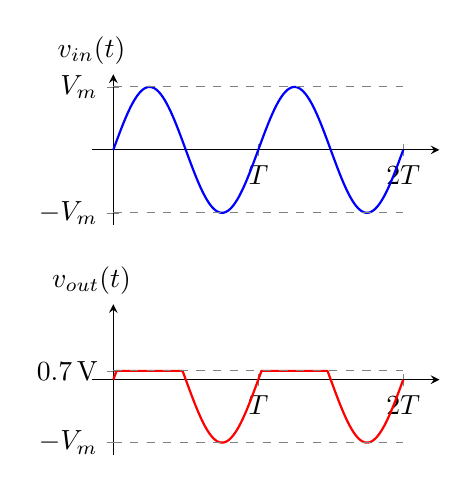
\begin{tikzpicture}
			\begin{groupplot}[
				group style={
					group size=1 by 2,
					vertical sep=1.0cm,
				},
				width=6cm, height=3.5cm,
				axis lines=middle,
				xmin=-0.3, xmax=4.5,
				ymin=-6, ymax=6,
				xtick={0,2,4},
				xticklabels={$0$,$T$,$2T$},
				domain=0:4,
				samples=200,
				clip=false,
				]
				
				% ---------- PANEL 1: INPUT ----------
				\nextgroupplot[
				ylabel={$v_{in}(t)$},
				ylabel style={
					at={(axis description cs:0,1)},  % top-left corner of the axis
					anchor=south,
					rotate=0,
				},
				ytick={5,-5},
				yticklabels={$V_m$,$-V_m$},
				]
				\addplot[thick, blue] {5*sin(deg(pi*x))};
				\draw[dashed, gray] (axis cs:0,5) -- (axis cs:4,5);
				\draw[dashed, gray] (axis cs:0,-5) -- (axis cs:4,-5);
				
				% ---------- PANEL 2: OUTPUT (clipped) ----------
				\nextgroupplot[
				ylabel={$v_{out}(t)$},
				ylabel style={
					at={(axis description cs:0,1)},  % top-left corner of the axis
					anchor=south,
					rotate=0,
				},
				ytick={0.7,-5},
				yticklabels={$0.7\,\text{V}$,$-V_m$},
				samples=400,
				]
				\addplot[thick, red] {min(5*sin(deg(pi*x)), 0.7)};
				\draw[dashed, gray] (axis cs:0,0.7) -- (axis cs:4,0.7);
				\draw[dashed, gray] (axis cs:0,-5) -- (axis cs:4,-5);
				
			\end{groupplot}
		\end{tikzpicture}
		\caption{Positive clipper waveforms}
		\label{fig:wavePosClipper}	
	\end{subfigure}
	%	
	\caption{Diode clipper circuit with input and output waveforms}
	\label{fig:clipper-full}
\end{figure}
The positive portion of the input waveform is clipped off, hence the name positive clipper.
\paragraph{(c) Shunt (Parallel) Clipper -- Negative Clipper.}
Figure~\ref{fig:shunt_neg_clipper} shows a shunt negative clipper with the diode across the output, placed in the opposite polarity compared to the positive clipper. Whenever $v_{in} < -V_F$, the diode conducts and clamps the output near $-V_F$; for $v_{in} > -V_F$, the diode is OFF and $v_{out} = v_{in}\dfrac{R_L}{R_L+R}$. If $R_L \gg R$, $v_{out}\approx v_{in}$. The waveforms expected are as given in Fig.~\ref{fig:waveNegClipper}. 

\begin{figure}[htbp]
	\centering
	%	
	%	% ---------- LEFT: circuit ----------
	\begin{subfigure}{0.42\textwidth}
		\centering
		\begin{circuitikz}[american, scale=1.0, line width=0.8pt]
			\draw
			(0,0) to[sinusoidal voltage source, l=$v_{in}(t)$] (0,3)
			(0,3) to[R, l=$R$, *-*] (4,3)
			(4,3) to[short] (6,3)
			(4,3) to[D, l=$D$, *-*, invert] (4,0)
			(4,0) to[short, *-*] (0,0)
			(6,3) to[R, l=$R_L$, *-*] (6,0)
			(6,0) to[short] (4,0);
			\draw (6,3) to[short, -o] (6.7,3) node[right]{$v_{out}(t)$};
			\draw (6,0) to[short, -o] (6.7,0) node[right]{};
			\draw (0,0) node[ground]{};
		\end{circuitikz}
		\caption{Shunt negative clipper.}
		\label{fig:shunt_neg_clipper}
	\end{subfigure}
	\hfill
	%	% ---------- RIGHT: stacked plots ----------
	\begin{subfigure}{0.52\textwidth}
		\centering
		%	
		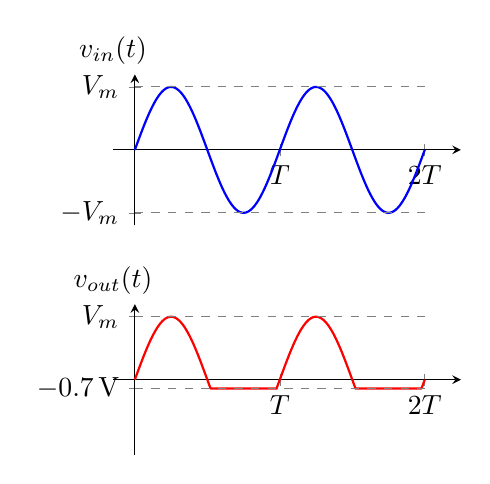
\begin{tikzpicture}
			\begin{groupplot}[
				group style={
					group size=1 by 2,
					vertical sep=1.0cm,
				},
				width=6cm, height=3.5cm,
				axis lines=middle,
				xmin=-0.3, xmax=4.5,
				ymin=-6, ymax=6,
				xtick={0,2,4},
				xticklabels={$0$,$T$,$2T$},
				domain=0:4,
				samples=200,
				clip=false,
				]
				
				% ---------- PANEL 1: INPUT ----------
				\nextgroupplot[
				ylabel={$v_{in}(t)$},
				ylabel style={
					at={(axis description cs:0,1)},  % top-left corner of the axis
					anchor=south,
					rotate=0,
				},
				ytick={5,-5},
				yticklabels={$V_m$,$-V_m$},
				]
				\addplot[thick, blue] {5*sin(deg(pi*x))};
				\draw[dashed, gray] (axis cs:0,5) -- (axis cs:4,5);
				\draw[dashed, gray] (axis cs:0,-5) -- (axis cs:4,-5);
				
				% ---------- PANEL 2: OUTPUT (clipped) ----------
				\nextgroupplot[
				ylabel={$v_{out}(t)$},
				ylabel style={
					at={(axis description cs:0,1)},  % top-left corner of the axis
					anchor=south,
					rotate=0,
				},
				ytick={-0.7,5},
				yticklabels={$-0.7\,\text{V}$,$V_m$},
				samples=400,
				]
				\addplot[thick, red] {max(-0.7, 5*sin(deg(pi*x)))};
				\draw[dashed, gray] (axis cs:0,-0.7) -- (axis cs:4,-0.7);
				\draw[dashed, gray] (axis cs:0,5) -- (axis cs:4,5);
				
			\end{groupplot}
		\end{tikzpicture}
		\caption{Negative clipper waveforms}
		\label{fig:waveNegClipper}	
	\end{subfigure}
	%	
	\caption{Diode clipper circuit with input and output waveforms}
	\label{fig:negClipper-full}
\end{figure}
The negative portion of the input waveform is clipped off, hence the name negative clipper.
\paragraph{(d) Biased Clippers.}
A DC bias source $V_R$ in series with the diode (Figure~\ref{fig:biased_clipper}) shifts the clipping level from $V_F$ to $(V_R + V_F)$ or $(V_R - V_F)$, depending on polarity. This allows the clipping level to be set anywhere on the waveform. There are two ways to achieve the biasing. One is to provide a direct dc source. The other is to use a Zener diode or series combination of diodes to achieve the bias level.

\begin{figure}[h!]
	\centering
	\begin{circuitikz}[american, scale=1.0, line width=0.8pt]
		\draw
		(0,0) to[sinusoidal voltage source, l=$v_{in}(t)$] (0,3)
		(0,3) to[R, l=$R$, *-*] (3,3)
		(3,3) to[short] (4,3)
		(3,3) to[D, l=$D$, *-*] (3,1.5)
		(3,1.5) to[battery1, l=$V_R$] (3,0)
		(3,0) to[short, *-*] (0,0)
		;
		\draw (4,3) to[short, -o] (4.7,3) node[right]{$v_{out}(t)$};
		\draw (3,0) to[short, -o] (4.7,0) node[right]{};
		\draw (0,0) node[ground]{};
	\end{circuitikz}
	\caption{Biased shunt clipper. Output is clipped at approximately $V_R + V_F$.}
	\label{fig:biased_clipper}
\end{figure}
\begin{figure}[htbp]
	\centering
	\begin{subfigure}{0.42\textwidth}
		\centering
			\begin{circuitikz}[american, scale=1.0, line width=0.8pt]
			\draw
			(0,0) to[sinusoidal voltage source, l=$v_{in}(t)$] (0,3)
			(0,3) to[R, l=$R$, *-*] (3,3)
			(3,3) to[short] (4,3)
			(3,3) to[D, l=$D$, *-*] (3,1.5)
			(3,1.5) to[battery1, l=$V_R$] (3,0)
			(3,0) to[short, *-*] (0,0)
			;
			\draw (4,3) to[short, -o] (5,3) node[right]{$v_{out}(t)$};
			\draw (3,0) to[short, -o] (5,0) node[right]{};
			\draw (4.5,3) to [R, l=$R_L$, *-*] (4.5,0);
			\draw (0,0) node[ground]{};
		\end{circuitikz}
		\caption{Biased positive clipper with dc source bias.}
		\label{fig:biasedSourceClipper}
	\end{subfigure}
	\hfill
	\begin{subfigure}{0.42\textwidth}
		\centering
		\begin{circuitikz}[american, scale=1.0, line width=0.8pt]
			\draw
			(0,0) to[sinusoidal voltage source, l=$v_{in}(t)$] (0,3)
			(0,3) to[R, l=$R$, *-*] (3,3)
			(3,3) to[short] (4,3)
			(3,3) to[D, l=$D$, *-*] (3,1.5)
			(3,1.5) to[zzDo, l=$V_Z$, invert] (3,0)
			(3,0) to[short, *-*] (0,0)
			;
			\draw (4,3) to[short, -o] (5,3) node[right]{$v_{out}(t)$};
			\draw (3,0) to[short, -o] (5,0) node[right]{};
			\draw (4.5,3) to [R, l=$R_L$, *-*](4.5,0);
			\draw (0,0) node[ground]{};
		\end{circuitikz}
		\caption{Biaed positive clipper with Zener diode for biasing.}
		\label{fig:biasedZenerClipper}
	\end{subfigure}
	\caption{Biased Positive Clipper Configurations}
\end{figure}
Fig.~\ref{fig:biasedSourceClipper} shows a biased positive clipper with a dc bias. Fig.~\ref{fig:biasedZenerClipper} shows the implementation with a Zener diode. The clipping levels are $V_R+V_F$ and $V_Z+V_F$ respectively. Fig.~\ref{fig:biasedClipperWaves} shows the sample waveforms. 
\begin{figure}[h!]
	\centering
	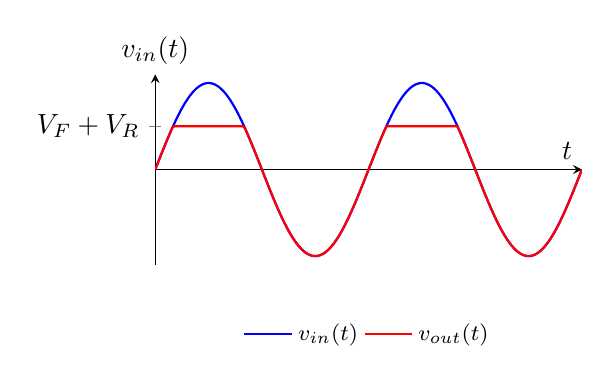
\begin{tikzpicture}
		\begin{axis}[
			width=7cm, height=4cm,
			xlabel={$t$}, 
			axis lines=middle,
			ymin=-2.2, ymax=2.2,
			ylabel={$v_{in}(t)$},
			ylabel style={
				at={(axis description cs:0,1)},  % top-left corner of the axis
				anchor=south,
				rotate=0,
			},
			xtick=\empty, ytick={1},
			yticklabels={$V_F+V_R$},
			domain=0:2, samples=200,
			legend style={draw=none, font=\footnotesize, at={(0.5,-0.25)}, anchor=north, legend columns=2}
			]
			\addplot[blue, thick] {2*sin(360*x)};
			\addlegendentry{$v_{in}(t)$}
			\addplot[red, thick] {min(2*sin(360*x), 1)};
			\addlegendentry{$v_{out}(t)$}
		\end{axis}
	\end{tikzpicture}
	\caption{Expected input and output waveforms for the biased positive clipper of Figure~\ref{fig:biasedSourceClipper}: the output is flattened above $V_F$.}
	\label{fig:biasedClipperWaves}
\end{figure}

In a similar way, a \textbf{Biased Negative Clipper} can be implemented by reversing the diode polarity. The figures~\ref{fig:biasedSourceClipperNeg} and \ref{fig:biasedZenerClipperNeg} show the circuit implementations.

\begin{figure}[htb]
	\centering
	\begin{subfigure}{0.42\textwidth}
		\centering
		\begin{circuitikz}[american, scale=1.0, line width=0.8pt]
			\draw
			(0,0) to[sinusoidal voltage source, l=$v_{in}(t)$] (0,3)
			(0,3) to[R, l=$R$, *-*] (3,3)
			(3,3) to[short] (4,3)
			(3,3) to[D, l=$D$,invert, *-*] (3,1.5)
			(3,1.5) to[battery1, l=$V_R$] (3,0)
			(3,0) to[short, *-*] (0,0)
			;
			\draw (4,3) to[short, -o] (5,3) node[right]{$v_{out}(t)$};
			\draw (3,0) to[short, -o] (5,0) node[right]{};
			\draw (4.5,3) to [R, l=$R_L$, *-*] (4.5,0);
			\draw (0,0) node[ground]{};
		\end{circuitikz}
		\caption{Biased negative clipper with dc source bias.}
		\label{fig:biasedSourceClipperNeg}
	\end{subfigure}
	\hfill
	\begin{subfigure}{0.42\textwidth}
		\centering
		\begin{circuitikz}[american, scale=1.0, line width=0.8pt]
			\draw
			(0,0) to[sinusoidal voltage source, l=$v_{in}(t)$] (0,3)
			(0,3) to[R, l=$R$, *-*] (3,3)
			(3,3) to[short] (4,3)
			(3,3) to[D, l=$D$,invert, *-*] (3,1.5)
			(3,1.5) to[zzDo, l=$V_Z$] (3,0)
			(3,0) to[short, *-*] (0,0)
			;
			\draw (4,3) to[short, -o] (5,3) node[right]{$v_{out}(t)$};
			\draw (3,0) to[short, -o] (5,0) node[right]{};
			\draw (4.5,3) to [R, l=$R_L$, *-*](4.5,0);
			\draw (0,0) node[ground]{};
		\end{circuitikz}
		\caption{Biaed negative clipper with Zener diode for biasing.}
		\label{fig:biasedZenerClipperNeg}
	\end{subfigure}
	\caption{Biased Negative Clipper Implementations}
	\label{fig:biasedNegClipperCkts}
\end{figure}
The sample waveforms for the biased negative clipper are as shown in Fig.~\ref{fig:biasedNegClipperWaves}.

\begin{figure}[htb]
	\centering
	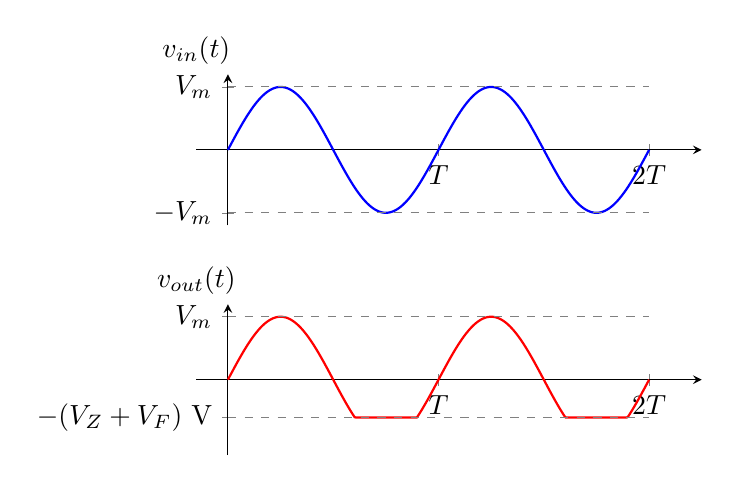
\begin{tikzpicture}
		\begin{groupplot}[
			group style={
				group size=1 by 2,
				vertical sep=1.0cm,
			},
			width=8cm, height=3.5cm,
			axis lines=middle,
			xmin=-0.3, xmax=4.5,
			ymin=-6, ymax=6,
			xtick={0,2,4},
			xticklabels={$0$,$T$,$2T$},
			domain=0:4,
			samples=200,
			clip=false,
			]
			
			% ---------- PANEL 1: INPUT ----------
			\nextgroupplot[
			ylabel={$v_{in}(t)$},
			ylabel style={
				at={(axis description cs:0,1)},  % top-left corner of the axis
				anchor=south,
				rotate=0,
			},
			ytick={5,-5},
			yticklabels={$V_m$,$-V_m$},
			]
			\addplot[thick, blue] {5*sin(deg(pi*x))};
			\draw[dashed, gray] (axis cs:0,5) -- (axis cs:4,5);
			\draw[dashed, gray] (axis cs:0,-5) -- (axis cs:4,-5);
			
			% ---------- PANEL 2: OUTPUT (clipped) ----------
			\nextgroupplot[
			ylabel={$v_{out}(t)$},
			ylabel style={
				at={(axis description cs:0,1)},  % top-left corner of the axis
				anchor=south,
				rotate=0,
			},
			ytick={-3,5},
			yticklabels={$-(V_Z+V_F)\ \text{V}$,$V_m$},
			samples=400,
			]
			\addplot[thick, red] {max(-3, 5*sin(deg(pi*x)))};
			\draw[dashed, gray] (axis cs:0,-3) -- (axis cs:4,-3);
			\draw[dashed, gray] (axis cs:0,5) -- (axis cs:4,5);
			
		\end{groupplot}
	\end{tikzpicture}
	\caption{Biased Negative Clipper Waveforms (For Zener based biasing)}
	\label{fig:biasedNegClipperWaves}
\end{figure}

\paragraph{(Double (Two-Level) Clipper or Slicer.}
Two diodes, oppositely poled and biased at $V_{R1}$ and $V_{R2}$, in parallel (Figure~\ref{fig:double_clipper}), clip both the positive peak above $(V_{R1}+V_F)$ and the negative peak below $-(V_{R2}+V_F)$, producing a trapezoidal output for a sinusoidal input of sufficient amplitude. This circuit is also known as a `slicer'. 

\begin{figure}[hbtp]
	\centering
	\begin{subfigure}{0.4\textwidth}
		\centering
		\begin{circuitikz}[american, scale=1.0, line width=0.8pt]
			\draw
			(0,0) to[sinusoidal voltage source, l=$v_{in}(t)$] (0,3)
			(0,3) to[R, l=$R$, *-*] (2.8,3)
			(2.8,3) to[short] (5,3)
			(2.8,3) to[D, l=$D_1$, *-] (2.8,1.8)
			(2.8,1.8) to[battery1, l=$V_{R1}$, *-*] (2.8,0)
			(2.8,0) to[short] (0,0)
			(4.4,3) to[D, l=$D_2$, invert, *-*] (4.4,1.8)
			(4.4,1.8) to[battery1, l=$V_{R2}$, invert] (4.4,0)
			(4.4,0) to[short, -*] (0,0)
			;
			\draw (4.4,3) to[short, -o] (6,3) node[right]{$v_{out}(t)$};
			\draw (4.4,0) to [short, -o] (6,0) node[right]{};
			\draw (0,0) node[ground]{};
			\draw (5.8,3) to [R, l=$R_L$, *-*] (5.8,0);
		\end{circuitikz}
		\caption{Slicer Circuit}
		\label{fig:double_clipper}
	\end{subfigure}
	\begin{subfigure}{0.58\textwidth}
		\centering
		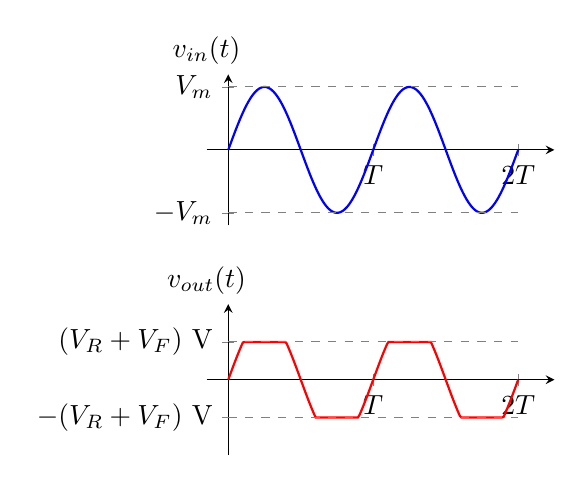
\begin{tikzpicture}
			\begin{groupplot}[
				group style={
					group size=1 by 2,
					vertical sep=1.0cm,
				},
				width=6cm, height=3.5cm,
				axis lines=middle,
				xmin=-0.3, xmax=4.5,
				ymin=-6, ymax=6,
				xtick={0,2,4},
				xticklabels={$0$,$T$,$2T$},
				domain=0:4,
				samples=200,
				clip=false,
				]
				
				% ---------- PANEL 1: INPUT ----------
				\nextgroupplot[
				ylabel={$v_{in}(t)$},
				ylabel style={
					at={(axis description cs:0,1)},  % top-left corner of the axis
					anchor=south,
					rotate=0,
				},
				ytick={5,-5},
				yticklabels={$V_m$,$-V_m$},
				]
				\addplot[thick, blue] {5*sin(deg(pi*x))};
				\draw[dashed, gray] (axis cs:0,5) -- (axis cs:4,5);
				\draw[dashed, gray] (axis cs:0,-5) -- (axis cs:4,-5);
				
				% ---------- PANEL 2: OUTPUT (clipped) ----------
				\nextgroupplot[
				ylabel={$v_{out}(t)$},
				ylabel style={
					at={(axis description cs:0,1)},  % top-left corner of the axis
					anchor=south,
					rotate=0,
				},
				ytick={-3,3},
				yticklabels={$-(V_R+V_F)\ \text{V}$,$(V_R+V_F)\ \text{V}$},
				samples=400,
				]
				\addplot[thick, red, samples=200] {max(-3, min(3, 5*sin(deg(pi*x))))};
				\draw[dashed, gray] (axis cs:0,-3) -- (axis cs:4,-3);
				\draw[dashed, gray] (axis cs:0,3) -- (axis cs:4,3);
			\end{groupplot}
		\end{tikzpicture}
		\caption{Input and output waveforms}
		\label{fig:slicerWaves}
	\end{subfigure}
	\caption{Slicer circuit and waveforms}
	\label{fig:slicer}
\end{figure}
Instead of DC biasing voltages, zener diodes can be used.
\subsection{Clamping Circuits}

A clamper consists of a diode, a capacitor, and a resistor, arranged so that the capacitor charges (through the low forward resistance of the diode) to the peak of the input during one half-cycle and holds this charge (discharging slowly through $R_L$, with $R_LC \gg T$) during the rest of the cycle, thereby shifting the DC level of the waveform. It essentially `clamps' the input signal up or down by the peak voltage. It is also called a DC restorer.

Mathematically, for an input signal given by $v){in}(t) = V_m\sin(\omega t)$, the clamper output is $v_o(t)= \pm V_m + V_m\sin(\omega t)$.

\paragraph{(a) Negative Clamper.}
Figure~\ref{fig:neg_clamper} shows a negative clamper, which shifts the waveform downward so that its positive peak is clamped at (approximately) $0\,\text{V}$ (or at $V_F$, accounting for diode drop).

\begin{figure}[h!]
	\centering
	\begin{subfigure}{0.4\textwidth}
		\centering
		\begin{circuitikz}[american, scale=1.20, line width = 0.85pt]
			\draw
			(0,0) to[sinusoidal voltage source, l=$v_{in}(t)$] (0,3)
			(0,3) to[cC, name = C, l=$C$, *-*] (2,3)
			(2,3) to[short] (3.5,3)
			(2,3) to[D, l=$D$, *-, mirror] (2,0)
			(2,0) to[short, -*] (0,0)
			(3.5,3) to[R, l=$R_L$] (3.5,0)
			(3.5,0) to [short, -*] (2,0);	
			\node [above left=1pt] at (C.left){\small $+$};	
		\end{circuitikz}
		\caption{Negative clamper circuit.}
		\label{fig:neg_clamper}
	\end{subfigure}
	\begin{subfigure}{0.52\textwidth}
		\centering
		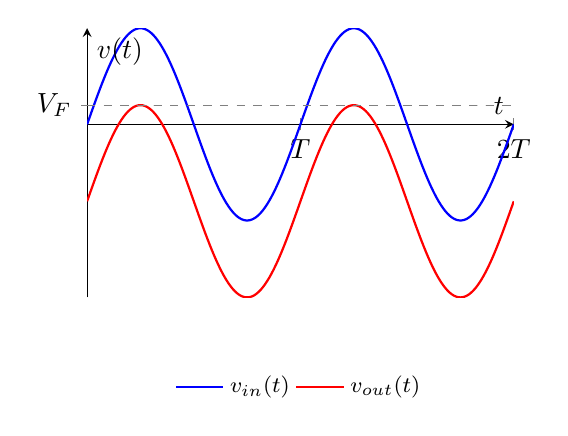
\begin{tikzpicture}
			\begin{axis}[
				width=7cm, height=5cm,
				xlabel={$t$}, 
				ylabel={$v(t)$},
				ylabel style={
				at={(axis description cs:0,1)},  % top-left corner of the axis
					anchor=south,
					rotate=90,
				},
				axis lines=middle,
				ymin=-4.5, ymax=2.5,
				xtick={0,1,2},
				xticklabels={$0$,$T$,$2T$},
				ytick={0.5},
				yticklabels={$V_F$},
				domain=0:2, samples=200,
				legend style={draw=none, font=\footnotesize, at={(0.5,-0.25)}, anchor=north, legend columns=2}
				]
				\addplot[blue, thick] {2.5*sin(360*x)};
				\addlegendentry{$v_{in}(t)$}
				\addplot[red, thick] {2.5*sin(360*x) - 2.5 + 0.5};
				\addlegendentry{$v_{out}(t)$}
				\addplot[gray, dashed] {0.5};
			\end{axis}
		\end{tikzpicture}
		\caption{Input and output waveforms for the negative clamper.}
		\label{fig:negWave_clamper}
	\end{subfigure}
	\caption{Negative Clamper: Circuit and waveforms}
\end{figure}

\paragraph{(b) Positive Clamper.}
Reversing the diode polarity (Figure~\ref{fig:pos_clamper}) clamps the negative peak of the waveform at approximately $0\,\text{V}$, shifting the entire waveform upward.

\begin{figure}[htbp]
	\centering
	\begin{subfigure}{0.42\textwidth}
		\centering
		\begin{circuitikz}[american, scale=1.0, line width=0.85pt]
			\draw
			(0,0) to[sinusoidal voltage source, l=$v_{in}(t)$] (0,3)
			(0,3) to[cC, name = C, l=$C$, invert, *-*] (2,3)
			(2,3) to[short] (3.5,3)
			(2,3) to[D, l=$D$, *-, invert] (2,0)
			(2,0) to[short, -*] (0,0)
			(3.5,3) to[R, l=$R_L$] (3.5,0)
			(3.5,0) to [short, -*] (2,0);	
			\node [above right=1pt] at (C.left){\small $+$};	
		\end{circuitikz}
		\caption{Positive clamper circuit (diode polarity reversed with respect to Figure~\ref{fig:neg_clamper}).}
		\label{fig:pos_clamper}
	\end{subfigure}
	\begin{subfigure}{0.52\textwidth}
		\centering
		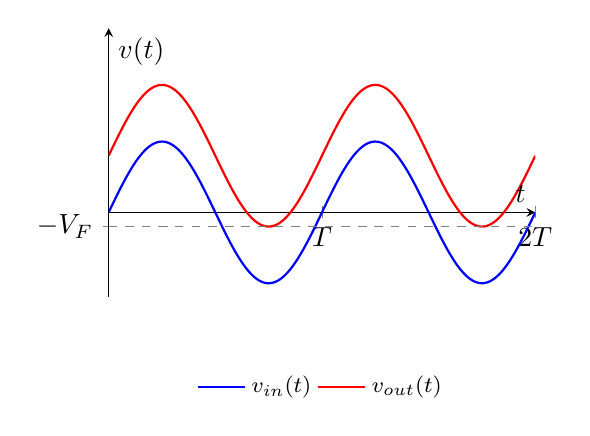
\begin{tikzpicture}
			\begin{axis}[
				width=7cm, height=5cm,
				xlabel={$t$}, 
				ylabel={$v(t)$},
				ylabel style={
					at={(axis description cs:0,1)},  % top-left corner of the axis
					anchor=south,
					rotate=90,
				},
				axis lines=middle,
				ymin=-3, ymax=6.5,
				xtick={0,1,2},
				xticklabels={$0$,$T$,$2T$},
				ytick={-0.5},
				yticklabels={$-V_F$},
				domain=0:2, samples=200,
				legend style={draw=none, font=\footnotesize, at={(0.5,-0.25)}, anchor=north, legend columns=2}
				]
				\addplot[blue, thick] {2.5*sin(360*x)};
				\addlegendentry{$v_{in}(t)$}
				\addplot[red, thick] {2.5*sin(360*x) + 2.5 - 0.5};
				\addlegendentry{$v_{out}(t)$}
				\addplot[gray, dashed] {-0.5};
			\end{axis}
		\end{tikzpicture}
		\caption{Input and output waveforms for the negative clamper.}
		\label{fig:posWaveClamper}
	\end{subfigure}
	\caption{Positive clamper: Circuit and waveforms}
\end{figure}
For an input sine wave of amplitude $V_m$, the steady-state clamped output ideally swings between:
\begin{align}
	\text{Negative clamper: } && v_{out} &\in [-2V_m + V_F,\; V_F], \label{eq:neg_clamp}\\
	\text{Positive clamper: } && v_{out} &\in [-V_F,\; 2V_m - V_F]. \label{eq:pos_clamp}
\end{align}
The time constant $R_L C$ must satisfy $R_L C \gg T$ (the input period) so that the capacitor voltage does not decay appreciably between successive charging peaks (poor choice of $R_L C$ leads to \emph{waveform tilt/sag}).


\section{Design Procedure}

\begin{enumerate}[label=(\alph*)]
	\item Select the operating signal's frequency and amplitude, $V_m$ and $f$. 
	\item For a biased clipper required to clip at a level $V_{clip}$, select $V_R = V_{clip} - V_F$ using a potential divider from the DC supply, or a battery/regulated source directly. A Zener diode may also be chosen, as described earlier.
	\item For a clamper, choose $C$ such that $R_L C \geq 10\,T$, where $T = 1/f$ is the period of the lowest input frequency to be used, so that the sag in output during discharge is limited to within an acceptable fraction (typically $< 5\%$) of $V_m$.
	\item Choose $R_L$ large enough to limit diode conduction current to a safe value, but small enough to keep $R_L C \gg T$ practical with standard capacitor values.
	\item \textbf{Selection of diodes}: For input frequencies less than 1 kHz, line frequency diodes such as 1N4001 may be used. For higher frequencies, these slow diodes are to be replaced with faster signal diodes such as 1N4148.
\end{enumerate}

\section{Experiment Procedure}

\begin{enumerate}[label=\arabic*.]
	\item Assemble the shunt positive clipper of Figure~\ref{fig:shunt_pos_clipper} on the breadboard. Set the function generator to a sine wave of frequency $1\,\text{kHz}$ and amplitude $5\,\text{V}_{pp}$.
	\item Connect DSO CH1 to $v_{in}$ and CH2 to $v_{out}$, with a common ground. Display both waveforms simultaneously and sketch/record them.
	\item Replace the shunt positive clipper with the shunt negative clipper. (Figure~\ref{fig:shunt_neg_clipper}). Record $v_{in}$ and $v_{out}$, and measure the clipping level from the DSO screen using the horizontal cursors.
	\item Repeat for the biased clipper (Figure~\ref{fig:biased_clipper}) for at least two values of $V_R$, and the double clipper (Figure~\ref{fig:double_clipper}).
	\item For each clipper configuration, tabulate the theoretically expected and experimentally measured clipping levels.
	\item Assemble the negative clamper (Figure~\ref{fig:neg_clamper}) using the design values of $R_L$ and $C$ computed in the Design Procedure. Apply the same sine wave and record $v_{in}$ and $v_{out}$ on the DSO, noting the DC shift and any tilt/sag in the output.
	\item Repeat for the positive clamper (Figure~\ref{fig:pos_clamper}).
	\item For each clamper, measure $V_{out,max}$ and $V_{out,min}$ using DSO cursors and compare with Equations~\eqref{eq:neg_clamp}--\eqref{eq:pos_clamp}.
	\item Vary the input frequency (e.g., to $100\,\text{Hz}$) while keeping $R_L C$ fixed, and observe/record the effect on clamper output tilt. Explain the observation.
\end{enumerate}

\subsection{Observation Tables}

\begin{table}[hb!]
	\centering
	\begin{tabular}{@{}lccccc@{}}
		\toprule
		Circuit & $V_{clip}$ (theory) & $V_{clip}$ (measured) & \% Error \\
		\midrule
		Shunt positive clipper &  &  &  \\
		Shunt negative clipper &  &  &  \\
		Biased positive clipper ($V_{R1}$) &  &  &  \\
		Biased megative clipper ($V_{Z}$) &  &  &  \\
		Double clipper (upper level) &  &  &  \\
		Double clipper (lower level) &  &  &  \\
		\bottomrule
	\end{tabular}
	\caption{Clipping circuits: theoretical vs. measured clipping levels.}
\end{table}

\begin{table}[hb!]
	\centering
	\begin{tabular}{@{}lcccc@{}}
		\toprule
		Circuit & $V_{out,max}$ (theory) & $V_{out,max}$ (meas.) & $V_{out,min}$ (theory) & $V_{out,min}$ (meas.) \\
		\midrule
		Negative clamper &  &  &  &  \\
		Positive clamper &  &  &  &  \\
		\bottomrule
	\end{tabular}
	\caption{Clamping circuits: theoretical vs. measured output extremes.}
\end{table}

\subsection{Precautions}
\begin{itemize}
	\item Observe correct diode polarity while assembling each circuit; an inverted diode produces the mirror-image (and often misleading) result.
	\item Do not exceed the diode's maximum forward current or reverse voltage ratings.
	\item Ensure a common ground between the function generator and both DSO channels.
	\item For clamping circuits, allow a few cycles for the capacitor to reach steady-state charge before recording the output.
	\item Use electrolytic capacitors, if used, with correct polarity as per the expected DC level at that node.
\end{itemize}
\begin{notebox}
	Experiment with higher frequency signals. What do you observe? Can you explain why circuit performance is not as expected at higher frequencies?
\end{notebox}
\subsection{Pre-Lab / Post-Lab Questions}
\begin{enumerate}[label=Q\arabic*.]
	\item Distinguish between series and shunt clipper configurations in terms of output impedance and loading effects.
	\item Derive the expression for the clipping level of the biased clipper of Figure~\ref{fig:biased_clipper} in terms of $V_R$ and $V_F$.
	\item Why must the time constant $R_L C$ of a clamper be much greater than the period of the input waveform? What happens if $R_L C$ is comparable to $T$?
	\item Sketch the output waveform of the double clipper (Figure~\ref{fig:double_clipper}) for an input triangular wave of amplitude greater than $(V_{R1}+V_{R2}+2V_F)$.
	\item A clamper is required to shift a $10\,\text{V}_{pp}$, $1\,\text{kHz}$ sine wave so that its output never goes negative. Design suitable values of $R_L$ and $C$, assuming a maximum permissible sag of $2\%$.
	\item Explain why a clipper is sometimes called a \emph{limiter} and give one practical application each of a clipper and a clamper in electronic systems.
	\item Why do clipper circuits do not perform as intended when diodes like 1N4001 are used, at higher frequencies, such as 50 kHz?
\end{enumerate}
\input{./experiments/expt2}
\input{./experiments/expt3}
\end{document}
